\chapter{Architektura oprogramowania i backend aplikacji}
\label{chap:BackendAplikacji}
\textit{Autor: Piotr Noga}
\par Niemniej ważnym elementem naszej pracy, od przedstawionego w poprzednim rozdziale interfejsu graficznego, było zaimplementowanie systemu, który byłby odpowiedzialny za przechowywanie wszelkich danych, które są wykorzystywane w trakcie działania aplikacji oraz za logikę biznesową, umożliwiającą działanie algorytmów zaprezentowanych w rozdziale \nameref{} czy też odpowiednie przetwarzanie informacji między użytkownikiem a wspomnianą wcześniej warstwą przechowywania danych.
Tę sekcję aplikacji przyjęło się w nomenklaturze informatycznej określać wyrazem z języka angielskiego "Backend" \cite{BackendDef}\cite{BackendDefArt}. Wyraz ten nie ma bezpośredniego tłumaczenia na język polski, stąd też w dalszej części tej pracy będzie on wykorzystywany, by określić wspomnianą powyżej warstwę programu.

\section{Architektura oprogramowania}
\label{sec:ArchitekturaOprogramowania}
Przed opisem backendu należy się zagłębić nad architekturą oprogramowania, gdyż to od niej tak naprawdę zależy, jak zostanie on zaimplementowany. Architektura ta wskazuje m.in. potrzeby jakie ma spełniać program oraz w jaki sposób powinien je realizować \cite{AO}.

\subsection{Architektura rozproszona}
\label{sec:Rozproszenie}
Jednym z założeń w naszej pracy jest zastosowanie architektury rozproszonej. Celem tego założenia jest to, aby można było zapisywać dane w taki sposób, żeby nie były one przechowywane tylko w jednym miejscu, gdyż mogłoby to doprowadzić do ich utraty, chociażby w przypadku awarii systemu. Taką potrzebę można spełnić poprzez zapisywanie danych w łańcuchach bloków \ang{Blockchain}, które byłyby dystrybuowane na inne komputery poprzez sieć P2P. 
\begin{figure}[!ht]
	\centering
		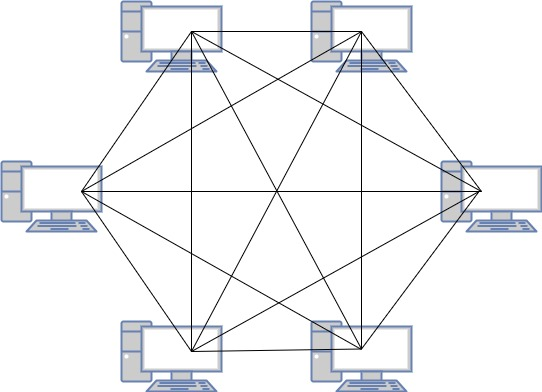
\includegraphics[width=0.3\textwidth]{Images/P2P.jpg}
	\caption{Sieć typu P2P}
	\label{fig:P2P}
\end{figure}
\newline Istnieje również alternatywne rozwiązanie tego założenia, mianowicie przechowywanie danych na różnych serwerach. Jest to w obecnych czasach częściej spotykane rozwiązanie, lecz nie spełnia ono kolejnej potrzeby, która jest opisana w następnej sekcji.
\begin{figure}[!ht]
	\centering
		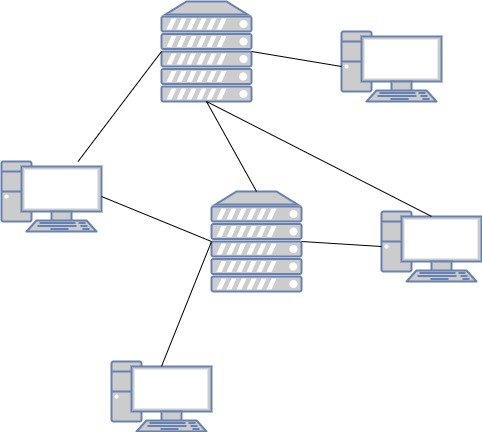
\includegraphics[width=0.3\textwidth]{Images/Siec_serwery.jpg}
	\caption{Sieć z różnymi serwerami}
	\label{fig:SiecSerwery}
\end{figure}
\newline

\subsection{Decentralizacja}
\label{sec:Decentralizacja}
Kolejnym wymogiem, jaki powinien być zrealizowany w naszej pracy, jest wykonanie aplikacji, która będzie działać w sposób zdecentralizowany. Oznacza to, że żaden użytkownik nie może mieć kontroli nad innymi, a co za tym idzie, nie ma żadnej scentraliozwanej jednostki, która może zarządzać przepływem danych w sieci. Z tego powodu drugie rozwiązanie, które zostało wspomniane w poprzedniej sekcji, czyli wykorzystanie różnych serwerów do przechowywania danych, nie może zostać wykorzystane w naszej implementacji. Wynika to z faktu, iż osoby zarządzające serwerami mogą arbitralnie zablokować niepożądanym w ich ocenie osobom dostęp do zasobów danych.


\section{Logika biznesowa}
\label{sec:LogikaBiznesowa}
Należy na początku poświęcić kilka słów wyjaśnienia, co kryje się pod pojęciem logika biznesowa. Jest to warstwa aplikacji odpowiedzialna za wykonywanie funkcji, które umożliwiają jej prawidłowe oraz spójne działanie. Kontroluje ona, co użytkownik może wykonać w aplikacji oraz definiuje warunki, jakie muszą zajść, by do danej czynności doszło. W logice biznesowej wykonywane są też przede wszystkim algorytmy, które zostały opisane w rozdziale \nameref{}. Implementując je w tej warstwie...  %--TODO--

\subsection{Komunikacja między użytkownikami}
\label{sec:Komunikacja}
Jednym z istotnych elementów naszego programu jest możliwość komunikowania się ze sobą użytkowników. W tym celu wykorzystaliśmy porozumiewanie się za pomocą protokołu HTTP. Wynika to z następujących zapotrzebowań:
\begin{itemize}
    \item bezpośrednia komunikacja między użytkownikami,
    \item dostosowanie przesyłanych danych w zależności od kontekstu,
    \item prostota zastosowania danego protokołu,
    \item szeroko dostępna dokumentacja protokołu.
\end{itemize}
Alternatywą do HTTP jest IPFS - InterPlanetary File System, który na pierwszy rzut oka wygląda na  lepsze rozwiązanie do naszej pracy, gdyż w przeciwieństwie do HTTP jest przystosowany do pracy w sieci rozproszonej, czym jest głównie reklamowany \cite{IPFS}. Nie wybraliśmy go jednak w naszej pracy ze względu na wcześniejsze doświadczenie z protokołem HTTP w poprzednich naszych projektach oraz na znikomą ilość pomocy dydaktycznej związanej z wykorzystaniem go w aplikacjach. 


\section{Przetwarzanie danych}
\label{sec:PrzetwarzanieDanych}